 
\documentclass[a4paper,12pt]{article}

\usepackage[utf8]{inputenc}
\usepackage[brazil]{babel}


\usepackage[left=2.5cm,right=2cm,top=2.5cm,bottom=2cm]{geometry}
\usepackage{graphicx}% Include figure files
%\usepackage{amsmath}
%\usepackage{mathtools} % % Loads amsmath
%\usepackage{bm}% bold math
\usepackage{amsmath}
%\usepackage{amssymb}
%\usepackage{amsthm}


%\usepackage{url}
\usepackage{hyperref}
\usepackage{url}
%
\usepackage{indentfirst}
\usepackage[inline]{enumitem}

\renewcommand{\baselinestretch}{1.2}


%opening
\title{Descrição do Modelo DELPHI}
            
\author{Marco A. Boselli}
\date{Instituto de Física \\
   Universidade Federal de Uberlândia \\
\today}




\begin{document}
 
\maketitle
 


\section{Modelo Preditivo}
\label{DELPHI}

A busca de modelos matemáticos que pudessem ajudar a quantificar e estudar a evolução de epidemias não é um assunto novo. O primeiro modelo de sucesso data de 1927 (Kermack e McKendrick)\cite{doi:10.1098/rspa.1927.0118}. Ao longo do tempo, este modelo recebeu releituras e complementações que dão origem aos novos modelos aplicados em estudo de viroses e mais recentemente aplicados a previsões na pandemia da Covid-19. 

Hoje temos duas linhas bem distintas de modelos matemáticos aplicados à epidemiologia, os modelos estocásticos e os modelos determinísticos. Os modelos estocásticos usam regressões e séries temporais e as previsões são feitas com base em distribuições estatísticas. Um exemplo dessa classe é o modelo do grupo do \textit{Imperial College COVID-19 Response Team}\cite{impirial1}. O modelo DELPHI\cite{delphi} se encaixa na classe dos modelos determinísticos, em que um conjunto de equações diferenciais é integrado num problema de valor de contorno\cite{2008elementary}. 

O modelo DELPHI usa o conjunto de equações diferenciais conhecidas como $SEIRD$ onde as variáveis  são 
\begin{itemize}
\item $S$ para suscetível,
\item $E$ para exposto,
\item $I$ para infectados,
\item $R$ para recuperados,
\item $D$ para óbitos.
\end{itemize}
Este conjunto é organizado da seguinte forma ,

\begin{align*}
 \frac{dS}{dt} & = - \alpha \gamma(t) S(t) I(t) \\
 \frac{dE}{dt} & = \alpha \gamma(t) S(t) I(t) \\
 \frac{dI}{dt} & = r_i E(t) - r_d I(t) \\
 \frac{d AR}{dt} & = r_d(1 - p_{dth})(1 - p_d) I(t) - r_{ri} AR(t) \\
 \frac{d DHR}{dt} & =  r_d (1 - p_{dth}) p_d p_h I(t) - r_{rh} DHR(t) \\
 \frac{d DQR}{dt} & = r_d (1 - p_{dth}) p_d (1 - p_h) I(t) - r_{ri} DQR(t) \\
 \frac{d AD}{dt} & =  r_d p_{dth} (1 - p_d) I(t) - r_{dth} AD(t) \\
 \frac{d DHD}{dt} & =  r_d p_{dth} p_{dph} I(t) - r_{dth} DHD(t) \\
 \frac{d DQD}{dt} & =  r_d p_{dth} p_d(1 - p_h) I(t) - r_{dth} DQD(t) \\
 \frac{d TH}{dt} & = r_d p_d p_h I(t)  \\
 \frac{d DD}{dt} & =  r_{dth} (DHD(t) + DQD(t)) \\
 \frac{d DT}{dt} & = r_d  p_d I(t) \\
 \frac{d R}{dt} & =  r_{ri} (AR(t) + DQR(t)) + r_{rh} DHR(t) \\
 \frac{d D}{dt} & =  r_{dth} (AD(t) + DQD(t) + DHD(t)) \, .
\end{align*}

Além das variáveis $SEIRD$ tradicionais descritas acima, o modelo apresenta o detalhamento: 
\begin{itemize}
\item Não detectados $(AR)$ \& $(AD)$: pessoas infectadas e em auto quarentena em casa devido a efeitos da doença. São variáveis para tratar casos não detectados. De alguma maneira, as pessoas se recuperam $(AR)$ e algumas morrem  $(AD)$.

\item Detectados Hospitalizados $(DHR)$ \& $(DHD)$: pessoas infectadas e testadas que necessitaram de hospitalização. Novamente a terminação R para recuperados e D para mortos.

\item Detectados em quarentena $(DQR)$ \& $(DQD)$: pessoas infectadas e em quarentena em casa. Segue a designação de $R$ e $D$.

\end{itemize}

A primeira equação do conjunto representa que a variação do número de pessoas suscetíveis ao longo do tempo cai (sinal negativo) com a taxa de infecção $\alpha$ a função auxiliar $\gamma$ e o contato entre os suscetíveis $S$ e os infectados $I$. Da mesma forma, a segunda equação representa que o número de expostos aumenta com o contato entre os suscetíveis $S$ e os infectados $I$. Para a equação dos infectados, a terceira, temos que seu número aumenta com o tempo na taxa $r_i$ com a qual os expostos $E$ se tornam doentes, e cai com a taxa $r_d$. Assim, cada uma das equações seguintes representam como cada variável aumenta com a sua respectiva taxa de variação.  Na última equação, o total de óbitos é a soma dos possíveis caminhos previstos no modelo.


Os parâmetros do modelo são:
\begin{itemize}
 \item $\alpha$ taxa de infecção (ajustado).
 
 \item $\gamma(t)$ medidas governamentais e respostas:
\[
  \gamma(t) = \frac{2}{\pi} \arctan \left( \frac{-(t - a)}{b}  \right) + 1
\]
usando os  a and b, é possível modelar o tempo de duração dos ajustes como restrição de comércio, distanciamento social, etc. Os parâmetros $a$ e $b$ são ajustados.

\item $r_d$ é a taxa de detecção.   $ r_d = \frac{log 2}{T_d}$,
 onde $T_d$ é a mediana do tempo para detecção (suposto ser 2 dias). Parâmetro fixo.

\item $r_i$ é a taxa de infecção deixando o tempo de incubação. 
  $r_i = \frac{log 2}{T_i}$  onde $T_i$ é o tempo mediano para deixar o período de incubação (suposto ser 5 dias).  Parâmetro fixo.

\item $r_{ri}$ é taxa de recuperação fora da hospitalização. 
   $r_{ri} = \frac{log 2}{T_{ri}}$, onde $T_{ri}$ é a mediana do tempo de recuperação dos casos não hospitalizados (suposto ser 10 dias). Parâmetro fixo.

\item $r_{rh}$ é taxa de recuperação sob hospitalização.
$r_{rh} = \frac{log 2}{T_{rh}}$ where $T_{rh}$, é a mediana do tempo de recuperação dos casos  hospitalizados (suposto ser 15 dias). Parâmetro fixo.

\item $r_{dth}$ é a taxa de morte.
 $r_{dth} = \frac{log 2}{T_{dth}}$, onde $T_{dth}$ é o tempo de espera do paciente até a morte. Parâmetro ajustado aos dados históricos.

\item $p_{dth}$ é a taxa de mortalidade. Parâmetro ajustado diretamente das curvas de óbitos.

\item $p_d$ é a porcentagem de casos detectados. Este valor é fixo em 0.2. Isto significa que para cada caso conhecido há 5 casos não detectados. 

\item $p_h$ é a porcentagem de detectados hospitalizados. Também é constante. 

\end{itemize}


Antes de passarmos para as previsões do modelo é importante entender a ação da função $\gamma(t)$ na modelagem. A interpretação correta dos resultados depende deste entendimento.
\begin{figure}[t]
 \centering
 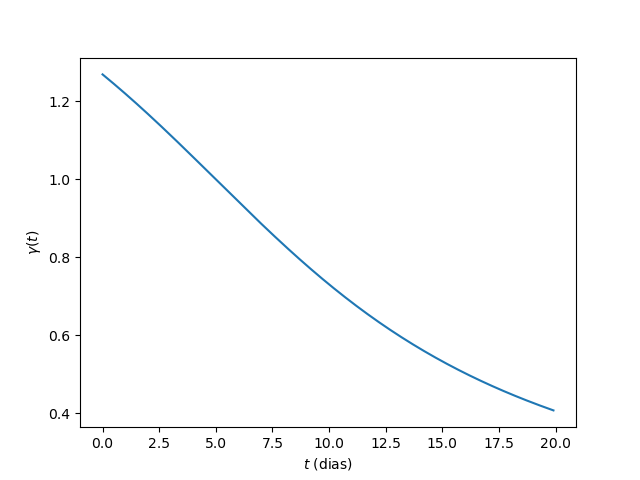
\includegraphics[width = 8cm]{figs/gamma_1.png}
 \caption{Formato típico da função $\gamma (t)$, aqui para os parâmetros $a = 20$ e $b = 5$. No processo de previsão estes números são ajustados.}
 \label{gamma}
\end{figure}


Na lista acima há parâmetros fixos e parâmetros ajustados. Os parâmetros fixos são aqueles que estão ligados à natureza humana, como tempo de incubação por exemplo, e não dependem de condições regionais. Os parâmetros ajustados são aqueles que vão carregar para o modelo as peculiaridades de cada população. O ajuste é feito com base nas curvas de óbitos acumulados (com peso maior) e nas curvas casos acumulados. O modelo considera o período a partir do centésimo caso acumulado detectado até a última atualização. O ajuste dos parâmetros é feito de forma a minimizar o quadrado da diferença entre a previsão o os casos reais. Os dados aqui usados são do Ministério da Saúde do Brasil \cite{minsaude}.  

\begin{figure}[t]
 \centering
 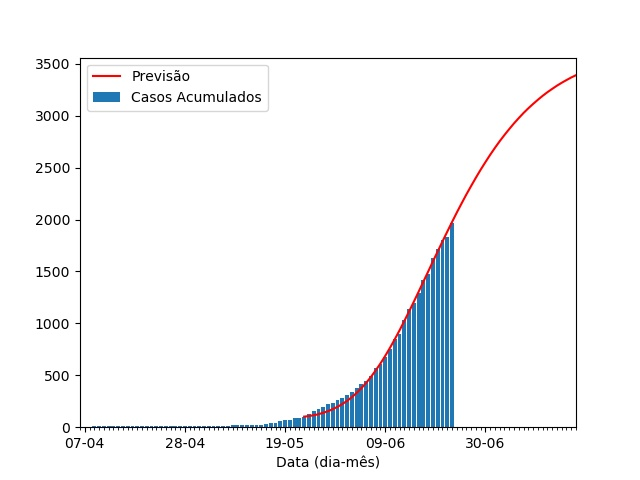
\includegraphics[width = 8cm]{figs/Fig_Brasil_MS_Dourados_casos_20200624_025dias.jpg}
 \caption{As barras azuis são número total de casos acumulados segundo o Ministério da Saúde para a cidade de Dourados - MS, e em vermelho a curva de previsão do modelo DELPHI para 25 dias.}
 \label{proj_casos}
\end{figure}


\begin{figure}[t]
 \centering
 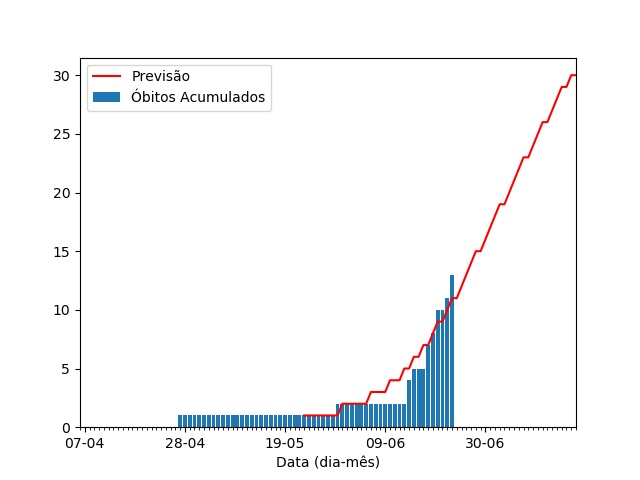
\includegraphics[width=8cm]{figs/Fig_Brasil_MS_Dourados_obitos_20200624_025dias.jpg}
 \caption{Gráfico de óbitos. Barras azuis são casos acumulados e curva vermelha previsão do modelo DELPHI para 25 dias.}
 \label{proj_obitos}
\end{figure}

Observando a Figura~\ref{gamma}, vemos que a função $\gamma(t)$ é sempre decrescente. Este fato captura o comportamento típico de uma epidemia viral onde a taxa de reprodução da doença normalmente cai com o número de infectados se tornando imunes ao longo do tempo, mas ela não é perfeita para a Covid-19. A adoção de medidas de isolamento social de fato contribui para a diminuição da taxa de reprodução e a função $\gamma$ como está é perfeita, porém a saída precoce do isolamento social pode fazer a taxa de reprodução voltar a crescer, e, nesse caso, a função necessita de ajuste, ou as previsões ficariam com tendência otimista. No modelo original, o grupo responsável pelo seu desenvolvimento acrescentou um módulo contando com as políticas adotadas em cada localidade. Esta implantação é restrita aos EUA, e não se aplica ao Brasil. Está em andamento um trabalho ainda inconcluso de adaptação desta estrutura de cálculo para o Brasil. Então, as previsões aqui apresentadas podem ter um viés otimista. 


A projeção, Figuras \ref{proj_casos} e \ref{proj_obitos}, aponta um aumento tanto no número de casos novos como no número de óbitos nos próximos dias. No ajuste dos parâmetros o modelo usa todos os dados do período a partir do dia do centésimo caso. Então, esta projeção é um apanhado de tudo que aconteceu anteriormente até o dia da último boletim. Para Dourados, o dia inicial é 23/5/2020 e o último boletim tem dados de 23/06/2020. O ajuste do modelo para ficou em acordo com casos reais neste período medido.

O comportamento social geral bem como a adoção ou ausência de medidas governamentais ficam embutidos nos parâmetros. O modelo permite previsões por quantos dias quisermos. Para a análise, foi escolhido um período de 25 dias para dar uma ideia do que acontece se nada mudar. Alterações do comportamento social atual podem alterar o padrão das curvas de crescimento, casos e óbitos, tanto para cima sem isolamento social, como para baixo com o isolamento  e consequentemente as respostas do modelo em rodadas futuras acompanharão estas mudanças.

Na Figura \ref{proj_casos} observamos que o comportamento de crescimento até hoje é exponencial. O mesmo comportamento vai se refletir na curva de óbitos, Figura \ref{proj_obitos}, que vinha mostrando um crescimento lento no número de mortes até 14/06/2020, e a partir daí dispara exponencialmente. Mantida esta tendência o número de óbitos pode dobrar em duas semanas.   


\bibliography{modelo.bib}{}
\bibliographystyle{plain}



\end{document}

